% !TEX root = paper.tex
\section{Evaluation}

LSD is evaluated against 12 C and C++ benchmarks, covering all the DOALLable
(showing at least speedup instead of slowdown) benchmarks from two
state-of-the-art automatic DOALL parallelization
papers~\cite{johnson:12:pldi,kim:12:cgo}. We also include one more benchmark
(179.art) from HELIX.

\begin{table*}
  % !TEX root = ../paper.tex
\small
\centering
\begin{tabular}{|l|c|c|l|l|}
\hline
Benchmarks & DOALL Coverage & Sequential Time & Arguments & Input    \\
\hline
doitgen    & 99.6\%  & 1034.86 & 768 768 768 & -  \\
\hline
enc-md5    & 100.0\% & 174.26    & 1000 & -  \\
\hline
covariance & 99.9\%  &     & 4096 4096 & -  \\
\hline
swaptions  & 100.0\% & 1546.29   & -ns 10000 -sm 40000 -nt 1 & -  \\
\hline
3mm  & 100.0\%       & 3515.78   & 4096 4096 4096 4096 4096                & -  \\
\hline
gemm       & 100.0\% & 1182.50   & 4096 4096 4096                    & -  \\
\hline
179.art    & 99.1\%  & 702.32    &
{\parbox[l]{5cm}{-scanfile c756hel.in \\-trainfile1 a10.img \\-trainfile2 hc.img\\ -stride 1 -startx 60 \\-starty 90 -endx 210 \\ -endy 240 -objects 10}} & input1   \\
\hline
dijkstra-dynsize & 99.7\%  &     & ../input3000/input3000.in 3000                & input300 \\
\hline
blackscholes & 99.7\% & 4702.20   & 1 in\_10M.txt out\_10M.txt                & ref      \\
\hline
2mm  & 100.0\%       & 2360.60   & 4096 4096 4096 4096               & -  \\
\hline
052.alvinn & 97.5\%  &     & 60000                 & input 1  \\
\hline
correlation & 99.7\%  & 914.39    & 4096 4096                   & - \\
\hline
\end{tabular}
  \caption{
    DOALL Coverage and Experiment Setting of Benchmarks
  }
  \label{tab:benchmark-list}
    \vspace{-5pt}
\end{table*}

The machine is using two 14-core Intel(R) Xeon(R)
CPU E5-2697 v3 CPU running at 2.60GHz (turbo-boost disabled) with 756GB of
memory. The operating system is Ubuntu 16.04.5 LTS with GCC 5.5 (version 5.5.0
20171010) and LLVM Compiler
Infrastructure (version 5.0.2).


\subsection{Parallelization Performance}
Figures Needed:
\begin{itemize}
\item General Speed Plot: With different cores (1-28), all benchmarks
\item Speedup Comparison: 24 cores performance compared with Privateer
Runtime breakdown (how to minimize the overhead?)

\end{itemize}

\begin{figure*}[htp]
  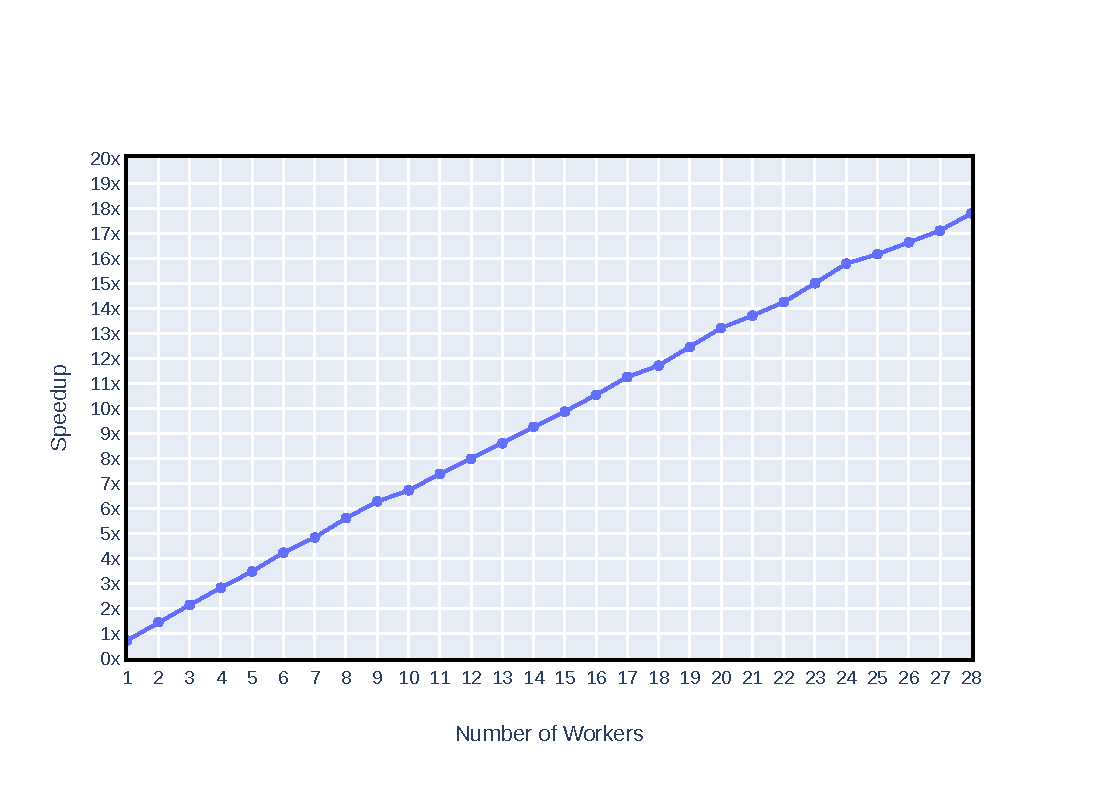
\includegraphics[width=\textwidth]{figures/3mm-scale-crop}
  \caption{3mm Speedup over Different Numbers of Cores}
  \label{fig:3mm-scale}
\end{figure*}

\subsubsection{Effect of parallelization on vectorization}

instrumentation kills vectorization


\subsection{Static Analysis and Enablers}
Figures Needed:
\begin{itemize}
\item CAF: with and without; no topping; with only BasicLoopAA and ScevAA
\item Coverage: Spec-DOALL percentage of coverage of each benchmark
\item Enablers: Enablers used for each benchmark
\item Optimization level: Performance with different optimization levels
\end{itemize}

Discussion Needed:

Present in a table for all the benchmarks which enablers were used

\subsection{Overhead Breakdown}

\begin{figure*}[htp]
  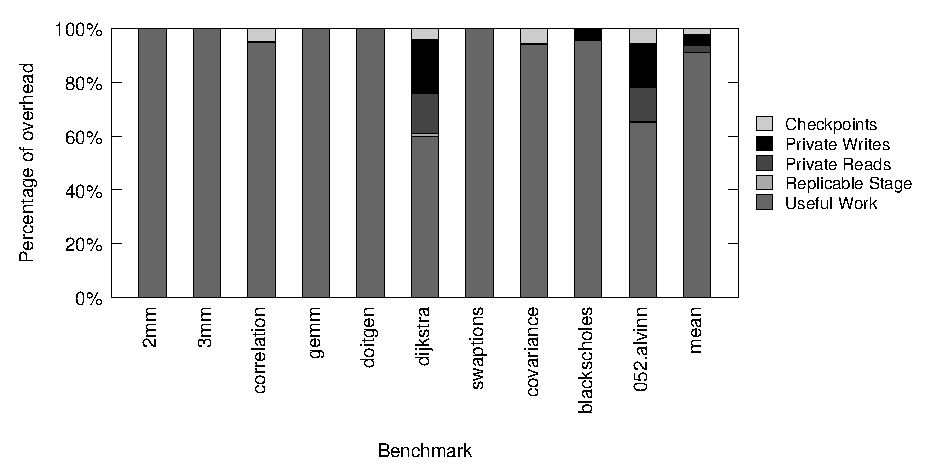
\includegraphics[width=0.9\textwidth]{figures/overheads}
\end{figure*}
\begin{figure*}[htp]
  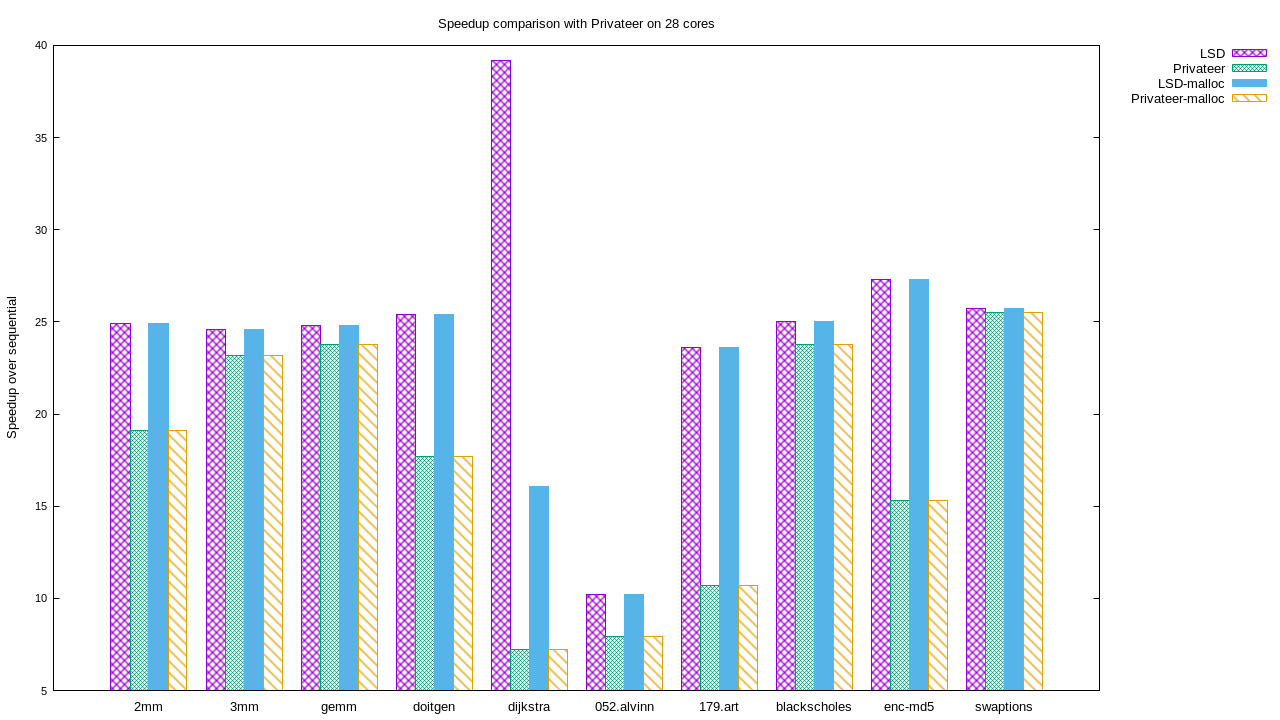
\includegraphics[width=0.9\textwidth]{figures/comparison}
\end{figure*}

\subsection{Power Consumption}

Power and energy stats here

